\documentclass[12pt]{article}

% setup link parameters (colors etc.)
\usepackage{hyperref}
\hypersetup{
	colorlinks   = true,
	citecolor    = gray
}

% math, symbols, theorem
\usepackage{amsmath}
\usepackage{amssymb}
\usepackage{amsthm}

% tikz for line drawings
\usepackage{tikz}
\usetikzlibrary{arrows}

% Subfigures
\usepackage{subfigure}

% algorithms
\usepackage[algonl,boxruled, lined]{algorithm2e}
\SetKwInput{kwInput}{Input}

% pin images/tables at certain position
\usepackage{float}

%\pagestyle{headings}
\title{Sample Report}
\author{Adarsh}
\date{}
\begin{document}
\maketitle

% Lets put a table of content here
\pagebreak
\hypersetup{linkcolor=black!40!orange}
\tableofcontents
\pagebreak
\hypersetup{linkcolor=blue!80!green}

\section{Problem 1}
Suppose we start with a currency $i_1$ and and trade our way through $i_2, i_3\dots$ to end up with a currency $i_k$. Its easy to see that if we start with one unit of $i_1$ currency then we will end up with $R[i_1,i_2].R[i_2,i_3]\dots R[i_{k-1},i_k]$ amount of currency $i_k$. We are more comfortable with addition than multiplication~\cite{tawarmalani2009allocating}. Hence, we can model the above conversion by taking $\log$ (base $e$) of $R[i,j]$ i.e. we start with $\log 1 = 0$ unit of currecy $i_1$ and end up getting $\log (R[i_1,i_2].R[i_2,i_3]\dots R[i_{k-1},i_k]) = \log R[i_1,i_2] + \log R[i_2,i_3]+\dots+\log R[i_{k-1},i_k]$ amount of currency $i_k$. Now further more, we want to choose set of currencies in our trade path such that we end up with largest units of $i_k$. Mathematically, we want to choose a set of currencies in our trading path such that $\log R[i_1,i_2] + \log R[i_2,i_3]+\dots+\log R[i_{k-1},i_k]$ is maximized or $ -\log R[i_1,i_2] - \log R[i_2,i_3]-\dots-\log R[i_{k-1},i_k]$ is minimized.


\section{Algorithm}
\begin{algorithm}[H]
	\kwInput{$G, s$}
	\KwResult{initialization}
	\For{ each vertex $v$ in $G$}{
		$d(v) = \infty$	\\
		$\pi(v) = null$ \\		
	}
	$d(s) = 0$
\caption{INITIALIZE($G,s$)}
\end{algorithm}   

\section{Tikzpicture}
\begin{center}
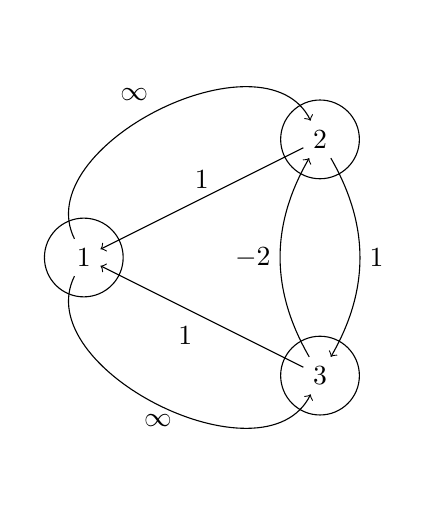
\begin{tikzpicture}[scale=1]
%\draw[help lines] (-2,2) grid (4,-4);
\draw (0,-1.5) circle (0.5cm);
\draw (3,0) circle (0.5cm);
\draw (3,-3) circle (0.5cm);
\node (n1) at (0, -1.5) {1};
\node (n2) at (3, 0) {2};
\node (n3) at (3, -3) {3};
\draw[bend left=90,->]  (n1) to node [auto] {$\infty$} (n2);
\draw[ ->]  (n2) to node [above] {$1$} (n1);
\draw[bend right=90,->]  (n1) to node [below] {$\infty$} (n3);
\draw[->]  (n3) to node [auto] {$1$} (n1);
\draw[bend left,->]  (n2) to node [auto] {$1$} (n3);
\draw[bend left,->]  (n3) to node [auto] {$-2$} (n2);
\end{tikzpicture} 
\end{center}

\section{Subfigures}
\begin{center}
	\begin{figure}[!h]
		\begin{tikzpicture}[scale=0.8]
		%\draw[help lines] (0,0) grid (8,8);
		\draw (0,0) -- (8.5,0) -- (8.5,8) -- (0,8) -- (0,0);
		\foreach \n in {(4,7.5),(4,7),(4,6.5),(4,6), (4,5.5), (4,0.5), (4,1), (4,1.5), (4,2), (4, 2.5)} {
			\draw[fill=red] \n circle [radius=0.1];
		}
		\foreach \n in {(4,5),(4,4.5),(4,4),(4,3.5), (4,3)} {
			\draw[fill=blue] \n circle [radius=0.1];
		}
		\node at (8,1) [below]{$(i)$};
		\end{tikzpicture}	
		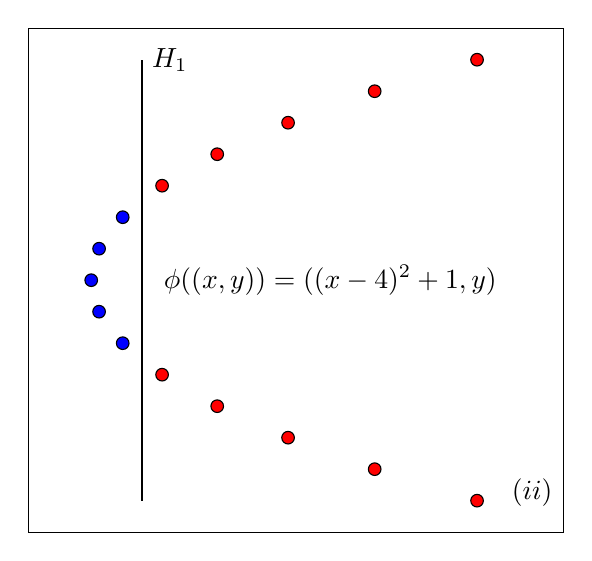
\begin{tikzpicture}[scale=0.8]
		%\draw[help lines] (0,0) grid (8,8);
		\draw (0,0) -- (8.5,0) -- (8.5,8) -- (0,8) -- (0,0);
		\foreach \n in {(7.125,7.5),(5.5,7),(4.125,6.5),(3,6), (2.125,5.5), (7.125,0.5), (5.5,1), (4.125,1.5), (3,2), (2.125, 2.5)} {
			\draw[fill=red] \n circle [radius=0.1];
		}
		\foreach \n in {(1.5,5),(1.125,4.5),(1,4),(1.125,3.5), (1.5,3)} {
			\draw[fill=blue] \n circle [radius=0.1];
		}
		\draw[thick] (1.81,0.5) -- (1.81,7.5);
		\node at (1.81,7.5) [right]{$H_1$};
		\node at (8,1) [below]{$(ii)$};
		\node at (2,4) [right]{$\phi((x,y)) = ((x-4)^2 + 1, y)$};
		\end{tikzpicture}
		\caption{Training Examples are not linearly separable} \label{fig:non-linear}
	\end{figure}
\end{center}

\section{External image}
% float package provides H option to pin figures/tables
\begin{figure}[H]
	\caption{A bird}
	\centering
	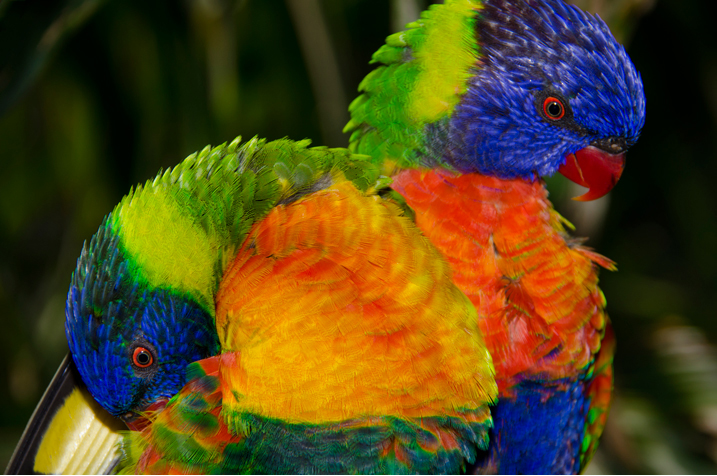
\includegraphics[scale=0.3]{../SampleImage/sample}
\end{figure}

\bibliography{report}
\bibliographystyle{apalike}
\end{document}